\section{Cayley Graphs}\label{cayley}

In this section, I'll first introduce Graph theory and then discuss about Cayley graphs. 


\subsection*{Graph Theory}
\begin{definition}
    A \textbf{graph} $G$ is a pair $(V, E)$ where V is a set and E is a subset of V (consisting of 2 elements).\\
The elements of set $V$ are called \textbf{vertices} and\\ the elements of set $E$ are called \textbf{edges} \cite{Tripi2017CayleyGO}.    
\end{definition}

So,  $V$ is the vertex set of $G$\\
and, $E$ is the edge set of $G$. 

\textbf{Notation}: Edges are written as $\{x, y\}$ and denoted by xy. Also, the edge $xy \in E$ is same edge as $yx \in E$. 
\begin{note} Adjacent vertices are called \textbf{neighbours}.   \end{note}
\begin{definition}
    If in a sequence $\left(x_1, x_2, ..., x_n\right)$ of vertices in a graph $G = (V, E)$, $x_i x_{i+1}$ is an edge for each $i=1,2, ..., n-1$ , then the sequence is called a \textbf{walk}. 
\end{definition}

\begin{definition}
    A walk whose vertices are distinct is called a \textbf{path}.
\end{definition}

\begin{definition}
    For $n \geq 3$, a path is called \textbf{cycle} if and only if $x_1x_n$ is also an edge in the graph. 
\end{definition}


\subsection*{Cayley Graph}

A Cayley Graph \cite{bartlett2014cayley,article} is a graph that describes the structure of a group. So, Cayley graphs are the geometric representation of groups. 

\begin{definition}
    Given a group  G and subset S ($S\subseteq G$), the \textbf{Cayley Graph} $[\Gamma(G,S)]$ is the unidirectional graph with vertex set (V) $=$ G and edge set (E) containing two vertices (x,y) if and only if $\exists$ some generator $s \in S$ such that $\boxed{x\cdot s=y}$
\end{definition}

\begin{note}
    $\Gamma(G,S)$ is connected if and only if S is generating set of G $[G = \langle S \rangle]$
. The generator (represented by arrows) point from one (represented by node) to another element only if it's generated by one of the generators. 
\end{note}

\begin{example}

Figure \ref{Figure_Cayleygraph} shows the Cayley graph of the group $(\mathbb{Z}_{6}, +)$ with the generator $1$. Each of the six elements of $\mathbb{Z}_6$ is represented by a node.

\begin{figure}[H]
\centering
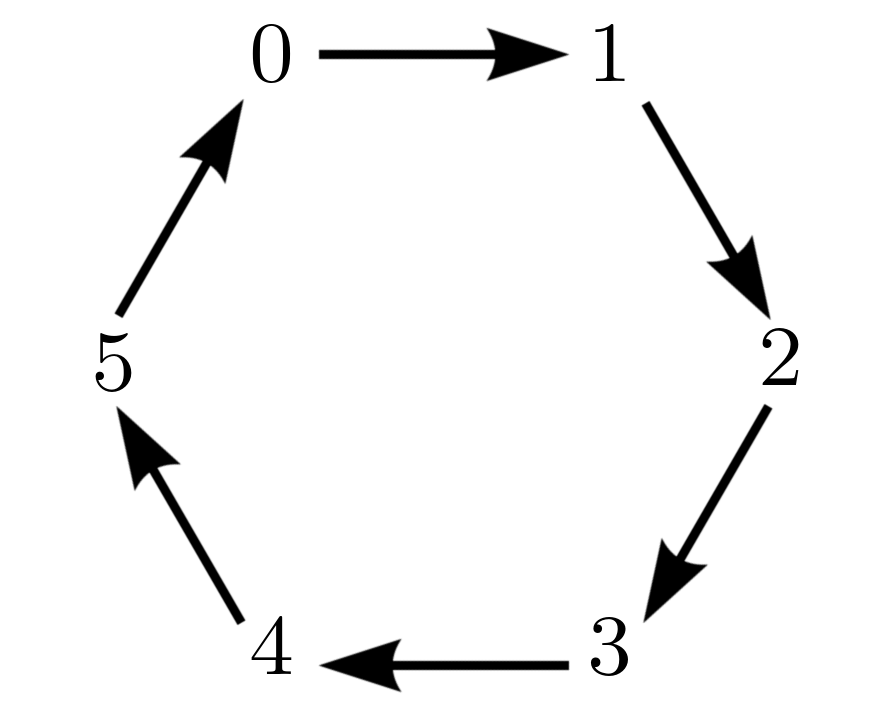
\includegraphics[scale=0.7]{Cayleygraph3.png}
\caption{Cayleygraph of $(\mathbb{Z}_ 6, +)$ with generator $1$}
\label{Figure_Cayleygraph}
\end{figure}
\end{example}

\begin{example}

Figure \ref{fig:z10} shows the Cayley graph of the group $(\mathbb{Z}_{10}, +)$ with the generator $\pm 1, \pm 2$.
   \begin{figure}[H]
    \centering
    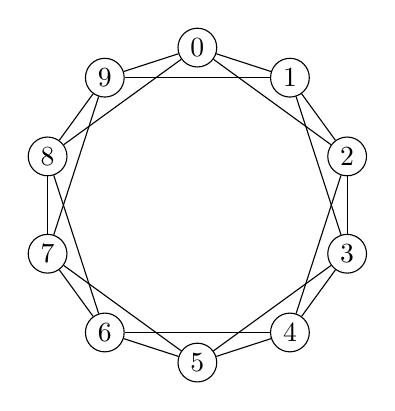
\begin{tikzpicture}[rotate=90]
        \tikzstyle{vertex}=[draw,thin,circle,fill=white,minimum size=14pt,inner sep=0pt]

        \draw (-0*360/10:2) node[vertex] (v1) {0};
        \draw (-1*360/10:2) node[vertex] (v2) {1};
        \draw (-2*360/10:2) node[vertex] (v3) {2};
        \draw (-3*360/10:2) node[vertex] (v4) {3};
        \draw (-4*360/10:2) node[vertex] (v5) {4};
        \draw (-5*360/10:2) node[vertex] (v6) {5};
        \draw (-6*360/10:2) node[vertex] (v7) {6};
        \draw (-7*360/10:2) node[vertex] (v8) {7};
        \draw (-8*360/10:2) node[vertex] (v9) {8};
        \draw (-9*360/10:2) node[vertex] (v10) {9};

        \draw (v2) -- (v1);
        \draw (v3) -- (v1);
        \draw (v3) -- (v2);
        \draw (v4) -- (v2);
        \draw (v4) -- (v3);
        \draw (v5) -- (v3);
        \draw (v5) -- (v4);
        \draw (v6) -- (v4);
        \draw (v6) -- (v5);
        \draw (v7) -- (v5);
        \draw (v7) -- (v6);
        \draw (v8) -- (v6);
        \draw (v8) -- (v7);
        \draw (v9) -- (v1);
        \draw (v9) -- (v7);
        \draw (v9) -- (v8);
        \draw (v10) -- (v1);
        \draw (v10) -- (v2);
        \draw (v10) -- (v8);
        \draw (v10) -- (v9);

    \end{tikzpicture}
    \caption{Cayley Graph of $(Z_{10})$ with the generating set $S= \{\pm 1, \pm 2 \}$}
    \label{fig:z10}
\end{figure}

\end{example}
\newpage

\begin{example}
Figure \ref{fig:D10} shows the Cayley graph of $D_{10}$ with the generating set $S= \{F, R, FR^{-1}\}$. 

 \begin{figure}[H]
\centering
    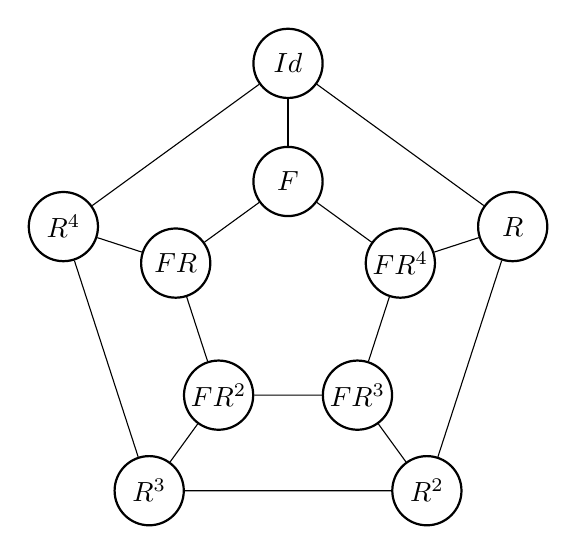
\begin{tikzpicture}[rotate=90,scale=1.5]
        \tikzstyle{vertex}=[draw,thick,circle,fill=white!60,minimum size=25pt,inner sep=0pt]

        \draw (-0*360/5:1) node[vertex] (v1) {$F$};
        \draw (-0*360/5:2) node[vertex] (v2) {$Id$};
        \draw (-1*360/5:1) node[vertex] (v3) {$FR^4$};
        \draw (-1*360/5:2) node[vertex] (v4) {$R$};
        \draw (-2*360/5:1) node[vertex] (v5) {$FR^3$};
        \draw (-2*360/5:2) node[vertex] (v6) {$R^2$};
        \draw (-3*360/5:1) node[vertex] (v7) {$FR^2$};
        \draw (-3*360/5:2) node[vertex] (v8) {$R^3$};
        \draw (-4*360/5:1) node[vertex] (v9) {$FR$};
        \draw (-4*360/5:2) node[vertex] (v10) {$R^4$};

        \draw (v2) -- (v1);
        \draw (v3) -- (v1);
        \draw (v4) -- (v2);
        \draw (v4) -- (v3);
        \draw (v5) -- (v3);
        \draw (v6) -- (v4);
        \draw (v6) -- (v5);
        \draw (v7) -- (v5);
        \draw (v8) -- (v6);
        \draw (v8) -- (v7);
        \draw (v9) -- (v1);
        \draw (v9) -- (v7);
        \draw (v10) -- (v2);
        \draw (v10) -- (v8);
        \draw (v10) -- (v9);
    \end{tikzpicture}
    \caption{Cayley Graph of $D_{10}$ with the generating set $S= \{F, R, FR^{-1}\}$}
    \label{fig:D10}
\end{figure}

\end{example}


My definition of a group operation with the group $(G_{2x2x2}, \scriptstyle * )$ and the set $C$ is : \\
If the Rubik's cube is in a configuration $C=(\sigma, x)$, making a move $M \in G_{2x2x2}$ will bring the cube into a new configuration  $C \cdot M$. 
\\
%Definition of a group operation with the group $(G_{2x2x2}, \scriptstyle*)$ and the set $C$:
%\begin{itemize}
%\item $ C \times G_{2x2x2} \rightarrow C$ with $(c, g) %\rightarrow c \cdot g $ [\textbf{Closure}]
%\item $c \cdot N = x$ for all $c \in C$ and the identity element $N \in G_{2x2x2}$ [\textbf{Identity}]
%\item $c \cdot (u \cdot v) = (c \cdot h) \cdot v$ for all $u, v \in G_{2x2x2}$ and $c \in C$ [\textbf{Associativity}]
%\end{itemize}
% \\
Suppose, the cube is in configuration $C$. Now when the move $M_1 \in G_{2x2x2}$ is made, the new configuration of the cube is $C \cdot M_1$. If another move $M_2 \in G_{2x2x2}$ is made, the new configuration of the cube is $(C \cdot M_1) \cdot M_2$. 
In other words: The cube started in configuration $C$ and the move $M_1 M_2$ was executed. I can also write the new configuration as $C \cdot (M_1 M_2)$ and therefore $(C \cdot M_1) \cdot M_2 = C \cdot (M_1 M_2)$. 

When we make the identity move $N$, the configuration of the cube is not changed. So $C \cdot N = C$. 
\\
In this case, the moves of the cube affect the configuration of the cube. 
%This is a right-hand operation because the elements of the group are on the right.
With Cayley graphs,  we'll have a group whose elements are the nodes of the graph. Here, the nodes of the graph are the elements of the group $(G_{2x2x2}, \scriptstyle*)$ and thus all possible moves. The edges correspond to the valid configurations of the cube, i.e. the set $C$. 

According to the paper \cite{cayleyrubik}, the Cayley graph of \Ttwo cube has $36, 74,160$ nodes which was computed on SUN-3 with 8 megabytes of storage in less than 60 CPU hours.





For more interesting Cayley graphs and deciphering the hidden beauties of finite groups [broadly speaking abstract algebra], one should definitely check this very beautiful paper by Matthew Macauley \cite{macauley2024revealing}. 
